\documentclass[a4paper,11pt]{article}
\usepackage{amssymb,microtype,natbib,graphicx}
\usepackage[font=small,labelfont=bf]{caption}
\usepackage[hidelinks]{hyperref}
\usepackage[T1]{fontenc}
\usepackage[english]{babel}
\usepackage{mathptmx}
\usepackage[onehalfspacing]{setspace}
\usepackage{abstract}
\setlength{\absleftindent}{0mm}
\setlength{\absrightindent}{0mm}

\newtheorem{theorem}{Theorem}
\author{Jakob Koscholke}
\bibpunct{([}{])}{;}{a}{}{}
\usepackage{sectsty}
\allsectionsfont{\normalsize\raggedright\centering}

\makeatletter
\renewcommand{\@seccntformat}[1]{\csname the#1\endcsname.\quad}
\makeatother


\title{How Prevalent is Transitivity-Failure in\\Bayesian Confirmation?}
\date{}

\begin{document}
\renewcommand{\abstractname}{\vspace{-\baselineskip}}

\maketitle

\begin{abstract}
\hrule\

\noindent It is a well-known fact among epistemologists and philosophers of science that transitivity can \emph{fail} for Bayesian confirmation. That is, it is possible that $A$ confirms $B$ and $B$ confirms $C$ while $A$ fails to confirm $C$. Still, there is a growing number of conditions in the literature under which this cannot happen, some of which are surprisingly weak. This raises the question how \emph{prevalent} the phenomenon of transitivity-failure is: perhaps, Bayesian confirmation is transitive \emph{in most cases}? The present paper aims at answering this and related questions with the help of a method known as Monte-Carlo integration. It also compares the prevalence of transitivity-failure with failures of adjacent inference patterns, some of which are known from non-monotonic reasoning and the logic of conditionals.

\ \hrule

%\begin{description}
%\item[Keywords.] Bayesian Confirmation Theory, Transitivity, Screening-off, Monte-Carlo Methods, Non-Monotonic Reasoning, Conditionals
%\end{description}
\end{abstract}



\section{Introduction}

According to Bayesian confirmation theory, a proposition $A$ \emph{confirms} another proposition $B$ relative to probability function $P$ if and only if $P(B|A)>P(B)$. This conception of confirmation was popularized by \cite{Carnap1950} but can be traced back to least \cite{Keynes1921}. And it is arguably \emph{the} most influential conception of confirmation currently on the market (for overviews see \citeauthor{Fitelson2001diss} [\citeyear{Fitelson2001diss}] or \citeauthor{Strevens2017} [\citeyear{Strevens2017}]). But it is a well-known fact among epistemologists and philosophers of science that confirmation, thus understood, is not transitive (see \citeauthor{Suppes1970} [\citeyear{Suppes1970}]). That is, the following inference pattern is invalid for Bayesian confirmation:\footnote{Bayesian confirmation is often contrasted with \emph{absolute} confirmation, i.e. sufficiently high conditional probability. I discuss transitivity-failure for absolute confirmation in \autoref{sec4}. For a recent alternative conception of confirmation see \citeauthor{Smith2016}'s \citeyearpar{Smith2016} idea of \emph{normic support}.} 

\begin{description}
\item[Transitivity.] If $A$ confirms $B$ and $B$ confirms $C$, then $A$ confirms $C$.
\end{description}

\noindent For an instance of transitivity-failure, consider drawing a single card from a well-shuffled standard deck and let $A$ state that the drawn card is a heart, $B$ that it is red and $C$ that it is a diamond (this example is due to \citeauthor{Roche2012b} [\citeyear{Roche2012b}]). We then have: 

\begin{itemize}
\item $P(B|A)=1>P(B)=1/2$
\item $P(C|B)=1/2>P(C)=1/4$
\item $P(C|A)=0<P(C)=1/4$
\end{itemize}

\noindent But the possibility of transitivity-failure does not mean that Bayesian confirmation is \emph{never} transitive. In fact, there is a growing number of conditions in the literature under which transitivity is valid. For instance, \cite{Suppes1970} pointed out that this is the case whenever $P(B|A)$ and $P(C|B)$ are maximal. And \cite{Hesse1970} uncovered a condition that guarantees the transitivity of Bayesian confirmation \emph{and} a restricted form of transitivity for absolute confirmation (see also \citeauthor{Koscholke2023} [\citeyear{Koscholke2023}]). \cite{Shogenji2003} later showed that Bayesian confirmation is transitive whenever $B$ screens-off $A$ and $C$ from each other (see also \citeauthor{Reichenbach1956} [\citeyear{Reichenbach1956}] or \citeauthor{Eellssober1983} [\citeyear{Eellssober1983}]). And \cite{Roche2012a} pointed out that screening-off can be weakened without compromising transitivity (see also \citeauthor{Suppes1986} [\citeyear{Suppes1986}]). Finally, \cite{Atkinson2021,Atkinson2021b} recently presented a new condition that is even weaker than the aforementioned. In fact, their condition can be made \emph{arbitrarily} weak and will still guarantee transitivity.

But if there are \emph{so many} conditions under which Bayesian confirmation is transitive, some of which are surprisingly weak, one might wonder how \emph{prevalent} instances of transitivity-failure actually are: could it be that Bayesian confirmation is transitive \emph{in most cases}? In this paper, I wish to answer this question with the help of a method known as Monte-Carlo integration. I will start by briefly explaining this method in \autoref{sec2} and continue by presenting the main results in \autoref{sec3}. In \autoref{sec4}, I present analogous results for absolute confirmation. And in \autoref{sec5} to \ref{sec7}, I compare the prevalence of transitivity-failure in Bayesian confirmation with the failure of adjacent inference patterns. I conclude in \autoref{conc}.\footnote{An anonymous referee remarked that the formulation `could it be that Bayesian confirmation is transitive \emph{in most cases}' is somewhat misleading since whether or not a relation is transitive depends on what happens \emph{in all cases}. To avoid confusion, the formulation should be `could it be that most cases in which $A$ confirms $B$ and $B$ confirms $C$ are also cases in which $A$ confirms $C$'. For ease of presentation, however, I will stick to the loose formulation above.}


\section{Monte-Carlo Integration}
\label{sec2}

\begin{figure}[t]
\centering
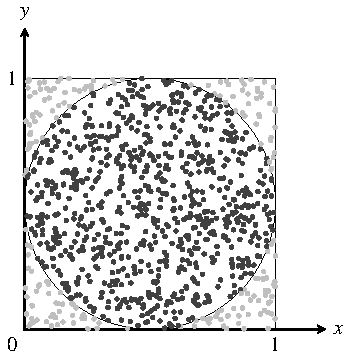
\includegraphics[scale=1]{monte.pdf} 
\caption{Approximating $\pi$ with 1000 randomly sampled points.}
\label{pi}
\end{figure}

Monte-Carlo integration is a computational method developed by \cite{Metropolis1949} to solve integration problems that are too complex to be solved analytically (see \citeauthor{Hammersley1964} [\citeyear{Hammersley1964}] or \citeauthor{Krauth2006} [\citeyear{Krauth2006}] for overviews). A well-known illustration of this method is the numerical approximation of $\pi$ \emph{via} integration over the area of a circle in a unit square, as shown in \autoref{pi}. One starts by picking a random sample of $n$ points from the unit square and then divides the number of points inside the circle by $n$. Since the area of a unit circle is $\pi/4$, one obtains an approximation of $\pi$ by multiplying the previous result by $4$. And the larger the random sample is, the closer the approximation will be to the real value. For example, for 1000 points one already obtains a circle area of around 79\% of the unit square thus a $\pi$ value of around 3.16.

\begin{table}[t]
\caption{Stochastic truth table.}
\centering
\begin{tabular}{rrrl} 
\hline
$A$ & $B$ & $C$ & $P$\\
\hline
0&0&0 & $p_1$ \\
0&0&1 & $p_2$\\
0&1&0 & $p_3$\\
0&1&1 & $p_4$\\
1&0&0 & $p_5$\\
1&0&1 & $p_6$\\
1&1&0 & $p_7$\\
1&1&1 & $p_8$\\
\hline
\end{tabular}
\label{stochastic}
\end{table} 

Now, determining $\pi$ numerically rather than analytically may seem like a mere math exercise. But it is very instructive, since our approach to determining the prevalence of transitivity-failure is almost identical. We did, however, not sample two-dimensional points from the Euclidean plane but eight-dimensional vectors from a hypervolume. The hypervolume represents the space of all probability functions over an algebra generated by three variables. Thus, each vector $(p_1,\ldots,p_8)$ with $p_i\geq 0$ and $\sum p_i=1$ is actually a probability function where each component is the probability assigned to the corresponding Boolean combination of our three variables $A$, $B$ and $C$. The exact correspondence is shown in \autoref{stochastic}, a so-called a \emph{stochastic truth-table} (for details see \citeauthor{Fitelson2008} [\citeyear{Fitelson2008}]). Since any such vector is either an instance of transitivity-failure or not, we can approximate the prevalence of transitivity-failure and transitivity-success by sampling as many vectors as possible. The results of this procedure are presented in the next section.\footnote{Monte-Carlo methods are well-established in the philosophical literature. \cite{Tentori2007} used them to test the agreement between Bayesian confirmation measures, \cite{Angere2007,Angere2008} and \cite{Koscholkeetal2018} for probabilistic coherence measures. \cite{Wagner2013} studied the prevalence of the so-called \emph{corroboration paradox} and \cite{Douven2015} investigated various closure principles for conditionals. \cite{Douven2018} used it to find sets of informative beliefs according to different belief-rules. And recently, \cite{Fitelson2021} used them to study various types of Simpson-paradoxical phenomena.}


\section{Transitivity-Failure in Bayesian Confirmation}
\label{sec3}

To ensure the numerical precision of our approximations, we sampled 10 million regular probability distributions from the set of all probability distributions on the algebra over three variables $A$, $B$ and $C$. These distributions were randomly generated using the Mersenne-Twister algorithm by \cite{Matsumoto1998} which corresponds to sampling from a uniform Dirichlet distribution on the unit 8-simplex with concentration parameters $\alpha_1,\ldots,\alpha_8$ equal to 1 (see \citeauthor{Kotz2000} [\citeyear{Kotz2000}]). This sample was then used to approximate two types of prevalence values of transitivity-failure:

\begin{itemize}
\item Conjunctive Prevalence: the proportion of cases in which $A$ confirms $B$ \emph{and} $B$ confirms $C$ \emph{and} $A$ fails to confirm $C$. Less formally, this quantity describes how prevalent instances of transitivity-failure are \emph{unconditionally}.

\item Conditional Prevalence: the prevalence of cases in which $A$ fails to confirm $C$ \emph{given that} $A$ confirms $B$ and $B$ confirms $C$. Less formally, this quantity describes how prevalent instances of transitivity-failure are \emph{conditional on} the transitivity-antecedent already being satisfied.
\end{itemize}

\begin{figure}[t]
\centering
\resizebox{\textwidth}{!}{
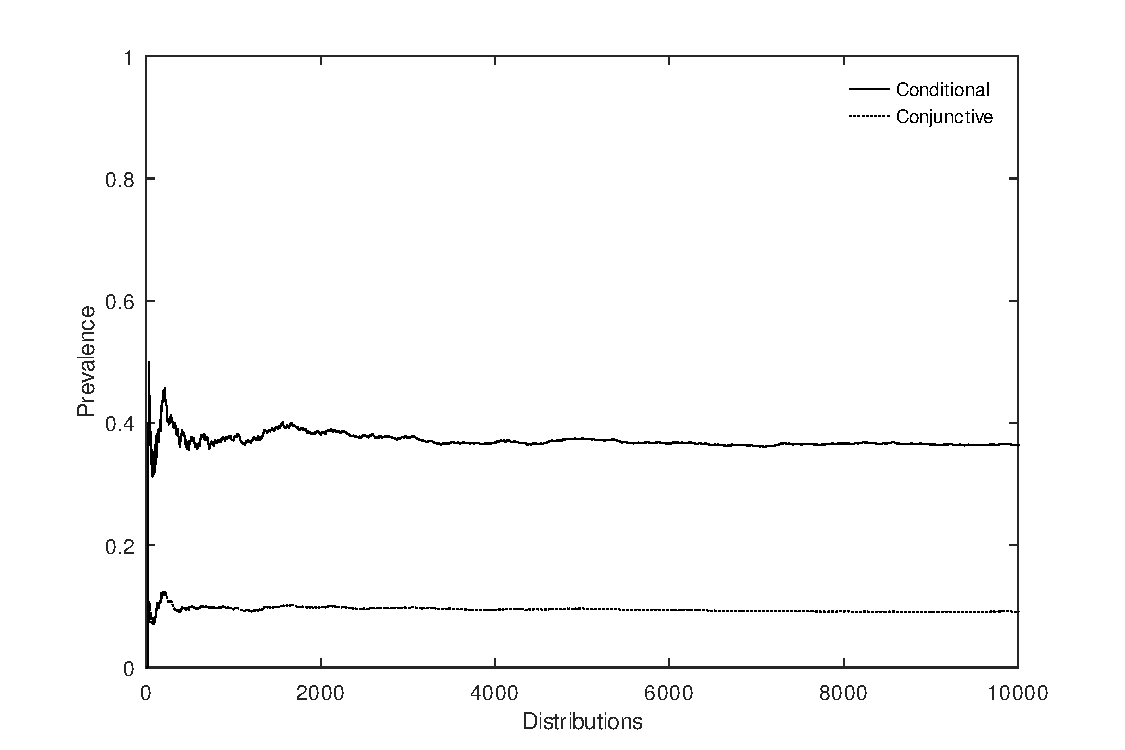
\includegraphics[]{trans_plot.pdf}}
\caption{Prevalence of transitivity-failure in Bayesian confirmation.}
\label{trans}
\end{figure}

\noindent As \autoref{trans} shows, the conjunctive prevalence of transitivity-failure quickly stabilized at around 9\%. This means that instances of transitivity-failure in Bayesian confirmation are less prevalent than instances of transi\-tivity-success. Notice, however, that the remaining 91\% of transitivity-success include \emph{trivial} cases where the antecedent of transitivity is violated or the consequent is satisfied. The conjunctive prevalence of \emph{non-trivial} instances of transitivity-success is around 16\%. 

The conditional prevalence stabilized at around 36\%. This means that if $A$ confirms $B$ and $B$ confirms $C$, inferring that $A$ confirms $C$ is more likely to be right than to be wrong, namely around 64\%. Still, since this is a rather high chance of error, it is fair to conclude that Bayesian confirmation is not transitive \emph{in most cases} (see also \citeauthor{Bamber2000}'s [\citeyear{Bamber2000}] idea of entailment with near surety).


\section{Transitivity-Failure in Absolute Confirmation}
\label{sec4}

Transitivity-failure occurs not only in \emph{Bayesian} but also in \emph{absolute} confirmation. On the latter conception, a proposition $A$ confirms another proposition $B$ relative to probability function $P$ if and only if $P(B|A)>\theta$, where $\theta$ is a threshold for high probability, presumably at least 1/2 (see \citeauthor{Carnap1950} [\citeyear{Carnap1950}]). For an example of transitivity-failure for $\theta=1/2$, consider again sampling from a well-shuffled standard deck of cards. This time, however, let $A$ state that the drawn card is a Two, Three, Four, Five, or Six, $B$ that the card is a Four, Five, Six, Seven, or Eight, and $C$ that the card is a Six, Seven, Eight, Nine, or Ten (this example is due to \citeauthor{Roche2017} [\citeyear{Roche2017}]). Here we have the following probabilities (and for even stronger counterexamples see \citeauthor{Douven2011} [\citeyear{Douven2011}]):

\begin{itemize}
\item $P(B|A)=3/5>\theta$
\item $P(C|B)=3/5>\theta$
\item $P(C|A)=1/5<\theta$
\end{itemize}

\noindent Still, there are also conditions under which absolute confirmation \emph{is} transitive. For instance, drawing on \citeauthor{Hesse1970}'s \citeyearpar{Hesse1970} work, \cite{Roche2017} pointed out that transitivity holds for absolute confirmation whenever $A$ is not negatively relevant for $C$ conditional on $B$ and the two conditional probabilities $P(B|A)$ and $P(C|B)$ are above the more demanding threshold for \emph{super-high} probability $\sqrt[2]{\theta}$. One might therefore also be interested in how prevalent transitivity-failure is in absolute confirmation. 

\begin{table}[t]
\caption{Transitivity-failure in absolute confirmation.}
\centering
\begin{tabular}{lccc}
\hline
Threshold $\theta $ & Conjunctive & Conditional\\
\hline
.5 &  0.05905960  & 0.23635440 \\
.7 &  0.01328240  & 0.28435759 \\
.9 &  0.00025400 & 0.30814024 \\
.95&   0.00001690 &  0.29911504 \\
.99&   0.00000000 &  0.00000000\\
\hline
\end{tabular}
\label{tab}
\end{table}

The results for different thresholds are shown in \autoref{tab}. It turns out that, just as in Bayesian confirmation, transitivity-failure in absolute confirmation is less prevalent than transitivity-success: the conjunctive prevalence ranges from 6\% to 0.001690\%, while the corresponding conjunctive prevalence of \emph{non-trivial} instances of transitivity-success ranges from 19\% to 0.0039600\%. The latter can be calculated from the values shown above. Importantly, the conditional prevalence of transitivity-failure is also lower than the corresponding prevalence of transitivity-success. This means that transitivity-style inferences are more likely to be right than to be wrong for absolute confirmation, namely around 70-76\%. And interestingly, this also means that transitivity-style inferences are more likely to be wrong for \emph{Bayesian} than for \emph{absolute} confirmation, namely around 36\% versus 24-30\%. 


\section{Varieties of Transitivity}
\label{sec5}

Transitivity-failure means that whenever $A$ confirms $B$ and $B$ confirms $C$, it does not follow that $A$ confirms $C$. But one might be tempted to infer that $A$ \emph{in conjunction with} $B$ confirms $C$. That is, one might think that the following inference pattern, also discussed by \cite{Douven2011}, is valid for Bayesian confirmation:

\begin{description}
\item[Conjunctive Transitivity.] If $A$ confirms $B$ and $B$ confirms $C$, then the conjunction $A\land B$ confirms $C$.
\end{description}

\noindent Similarly, one might be tempted to infer that $A$ confirms $C$ \emph{conditional on} $B$, that is $P(C|A\land B)>P(C|B)$. To the best of my knowledge, the resulting inference pattern has not yet been discussed in the literature: 
\begin{description}
\item[Conditional Transitivity.] If $A$ confirms $B$ and $B$ confirms $C$, then $A$ confirms $C$ conditional on $B$.
\end{description}

\noindent But our initial card example shows that both patterns are invalid for Bayesian confirmation. If $A$ is that the drawn card is a heart, $B$ that it is red and $C$ that it is a diamond, we have: 

\begin{itemize}
\item $P(B|A)=1>P(B)=1/2$
\item $P(C|B)=1/2>P(C)=1/4$ 
\item $P(C|A\land B)=0<P(C)=1/4<P(C|B)=1/2$
\end{itemize}


\noindent One might also wonder about the validity of another transitivity-like pattern known from non-monotonic reasoning (see \citeauthor{Kraus1990} [\citeyear{Kraus1990}]):

\begin{description}
\item[Cumulative Transitivity.] If $A$ confirms $B$ and $A\land B$ confirms $C$, then $A$ confirms \nolinebreak  $C$.%\footnote{Cumulative Transitivity, Reflexivity and Monotonicity entail Transitivity.}
\end{description}

\noindent But this pattern is also invalid for Bayesian confirmation. To see this, consider the following variation of our card example for absolute confirmation. Let $A$ state that the drawn card is a Two, Three, Four, Five, or Six, $B$ that the card is a Four, Five, Six, Seven, or Eight, and $C$ that the card is a Five, Six, Seven, Eight or Nine. We then have:

\begin{itemize}
\item $P(B|A)=3/5>P(B)=5/13$
\item $P(C|A\land B)=2/3>P(C)=5/13$ 
\item $P(C|A)=2/5<P(C)=5/13$
\end{itemize}

\noindent Interestingly, while each of the aforementioned transitivity-like patterns is invalid, there are significant differences between them: failures of conjunctive and cumulative transitivity are less prevalent than failures of conditional transitivity or standard transitivity; and somewhat surprisingly, conditional transitivity has the highest prevalence of failure. The exact values are shown in  \autoref{patterns}.\footnote{\cite{Freund1991} also discuss a variation of transitivity with a strengthened antecedent. When adapted to confirmation, it reads: 

\begin{description}
\item[Weak Transitivity.] If $A$ confirms $B$, $B$ confirms $C$ and $B$ does not confirm $\neg A$, then $A$ confirms $C$.
\end{description}

\noindent But for Bayesian confirmation, the added conjunct is already implied by the first conjunct of the antecedent.} 

\begin{table}[t]
\caption{Failure-prevalence for other inference patterns. Here, $>$ abbreviates Bayesian confirmation, a subscript indicates conditional confirmation. For an investigation of some of these patterns for absolute confirmation see \cite{Hawthorne1996} or \cite{Hawthorne2007}.}
\resizebox{\textwidth}{!}{
\begin{tabular}{llcc}
\hline
Label & Pattern & Conjunctive & Conditional\\
\hline
Transitivity & If $A>B$ and $B>C$, then $A>C$ & 0.090 &	0.359\\
Conjunctive Transitivity & If $A>B$ and $B>C$, then $A\land B>C$  & 0.056 &	0.226\\
Conditional Transitivity & If $A>B$ and $B>C$, then $A>_B C$ &  0.111 &	0.443\\
Cumulative Transitivity & If $A>B$ and $A\land B>C$, then $A>C$ & 0.056 &	0.225\\
Agglomeration & If $B>A$ and $B>C$, then $B>A\land C$ & 0.025 &	0.101\\
Cautious Monotonicity & If $B>A$ and $B>C$, then $B\land C>A$ & 0.057 &	0.226\\
Rational Monotonicity & If $B>A$ and $B\ngtr \neg C$, then $B\land C>A$ & 0.057 &	0.226\\
Corroboration & If $A>B$ and $C>B$, then $A>_C B$ and $C>_A B$ & 0.092 &	0.368\\
Amalgamation & If $A>B$ and $C>B$, then $A\lor C > B$ & 0.025 &	0.100\\
\hline
\end{tabular}}
\label{patterns}
\end{table}


\section{Agglomeration and Monotonicity}

On the Bayesian conception of confirmation, the antecedent of transitivity is equivalent to $B$ confirming $A$ and $C$ individually. And \cite{Reichenbach1956} famously showed that if additionally $B$ screens-off $A$ and $C$ from each other, it follows that $B$ confirms the conjunction $A\land C$. This corresponds to the following well-known inference pattern (see \citeauthor{Leitgeb2013lottery} [\citeyear{Leitgeb2013lottery}] for the label):

\begin{description}
\item[Agglomeration.] If $B$ confirms $A$ and $B$ confirms $C$, then $B$ confirms their conjunction $A\land C$.
\end{description}

\noindent And the antecedent of transitivity and of agglomeration are identical to the antecedent of the following weak form of monotonicity (see \citeauthor{Gabbay1985} [\citeyear{Gabbay1985}]):

\begin{description}
\item[Cautious Monotonicity.] If $B$ confirms $A$ and $B$ confirms $C$, then $B\land C$  confirms \nolinebreak $A$. 
\end{description}

\noindent And cautious monotonicity is closely related to another weak form of monotonicity known from the logic of conditionals (see \citeauthor{Lewis1973} [\citeyear{Lewis1973}]):

\begin{description}
\item[Rational Monotonicity.] If $B$ confirms $A$ and $B$ does not confirm $\neg C$, then $B\land C$ confirms $A$.
\end{description}

\noindent But all three inference patterns are invalid for Bayesian confirmation. To see this, simply reconsider our initial card example where $A$ is that the drawn card is a heart, $B$ that it is red and $C$ that it is a diamond. We then have:

\begin{itemize}
\item $P(A|B)=1/2>P(A)=1/4$
\item $P(C|B)=1/2> P(C)=1/4$ 
\item $P(A\land C|B)=P(A\land C)=0$
\end{itemize}


\noindent Despite their invalidity, however, each of the three patterns has a lower prevalence of failure than transitivity. In fact, agglomeration-failure has the lowest prevalence of all investigated patterns. See \autoref{patterns} for the precise values. 

\section{Corroboration and Amalgamation}
\label{sec7}

On the Bayesian conception of confirmation, the transitivity-antecedent is also equivalent to $A$ and $C$ individually confirming $B$. And \cite{Cohen1977} showed that if additionally two weak conditional independence conditions hold, it follows that $A$ and $C$ \emph{together} make $B$ more likely than they do \emph{individually}. This corresponds to the following inference pattern, also discussed by \cite{Wagner2013}:\footnote{For critical comments on Cohen's work see \cite{Oneill1982}, \cite{Falk1986} and \cite{Schlesinger1988}, but see also \cite{Cohen1982}, \cite{Cohen1986}, \cite{Cohen1991} and \cite{Wagner1991} for replies. \cite{AtkinsonManuscript} provide a nice overview.}
 
\begin{description}
\item[Corroboration.] If $A$ confirms $B$ and $C$ confirms $B$, then $A$ confirms $B$ conditional on $C$ and $C$ confirms $B$ conditional on $A$.
\end{description}

\noindent Whenever $A$ and $C$ confirm $B$ individually, one might also be tempted to infer that their disjunction $A\lor C$ confirms $B$. This corresponds to the following inference pattern (see \citeauthor{Smith2016} [\citeyear{Smith2016}] for the label):

\begin{description}
\item[Amalgamation.] If $A$ confirms $B$ and $C$ confirms $B$, then their disjunction $A\lor C$ confirms $B$.
\end{description}

\noindent But again, both aforementioned patterns are invalid for Bayesian confirmation. Our initial card example yields the following probabilities:

\begin{itemize}
\item $P(B| A)=1 > P(B)=1/2$
\item $P(B| C)=1 > P(B)=1/2$
\item $P(B|A\land C)$ is undefined and cannot be higher than $P(B|A)$ or $P(B|C)$
\item $P(B| A\lor  C)= P(B)=1/2$
\end{itemize}

\noindent Interestingly, while amalgamation-failure is less prevalent than transitivity-failure, corroboration-failure is significantly more prevalent than the latter. Arguably, this is due to the fact that the corroboration-consequent is a conjunction and thus more difficult to satisfy. The exact numbers are again shown in \autoref{patterns}.\footnote{The MATLAB code underlying these results is available upon request.}


\section{Conclusion}
\label{conc}

Bayesian confirmation may not be transitive, but the phenomenon of transi\-tivity-failure is much less common than one might expect: the results above show that it is less prevalent than trivial as well as non-trivial instances of transitivity-success. Still, this does not mean that Bayesian confirmation is transitive \emph{in most cases}: there is a non-negligible chance of error in transitivity-style inferences. And transitivity-failure is also more prevalent than failures of many adjacent inference patterns from non-monotonic reasoning and the logic of conditionals.

The above results can also be taken as an inspiration to further investigate the logic of Bayesian confirmation quantitatively rather than qualitatively. Scholars like \cite{Pearl1991} have complained that the Bayesian notion of confirmation ``in itself is too weak to yield interesting inferences'' \cite[][160]{Pearl1991}. But this is only true if interesting inferences are required to be classically valid. The quantitative picture is much more complex. Then, as we have seen above, the notion of Bayesian confirmation yields many interesting inferences with varying degrees of validity. And there are probably more than the ones examined here.\footnote{Do the results presented here mean that it is \emph{rational} to infer, for example, the conclusion that $A$ confirms $C$ from the premises that $A$ confirms $B$ and that $B$ confirms $C$? No. As the literature on the normativity of logic shows, it is already difficult enough to formulate rationality principles for \emph{valid} inferences (see \citeauthor{Steinberger2017} [\citeyear{Steinberger2017}]). Accordingly, we should be even more careful when thinking about the implications the results might have for the rationality of \emph{invalid} inferences. Thanks to an anonymous referee for pushing me to say a bit more about this.}


\section*{Acknowledgments}

This paper was written during a Visiting Scholarship at Stanford University in 2022. I am grateful to Krista Lawlor for sponsoring my visit to Stanford and to the Hamburg Research Academy for financial support. I also would like to thank Jeanne Peijnenburg, David Atkinson, Igor Douven and two anonymous referees for helpful feedback. Special thanks to Branden Fitelson for taking the time to discuss an earlier version of this paper. This work was funded by the German Research Foundation (DFG) as part of grant ZI 1824/1-1 to Alexandra Zinke.

\hfill

\begin{flushright}
\emph{Jakob Koscholke\\Goethe University Frankfurt\\
Koscholke@em.uni-frankfurt.de}
\end{flushright}


\begin{thebibliography}{}

\bibitem[Angere, 2007]{Angere2007}
Angere, S. [2007]:
\newblock `The defeasible nature of coherentist justification',
\newblock {\em Synthese}, \textbf{157}, pp. 321--335.

\bibitem[Angere, 2008]{Angere2008}
Angere, S. [2008]:
\newblock `Coherence as a heuristic',
\newblock {\em Mind}, \textbf{117}, pp. 1--26.

\bibitem[Atkinson and Peijnenburg, 2021a]{Atkinson2021}
Atkinson, D. and Peijnenburg, J. [2021a]:
\newblock `A new condition for transitivity of probabilistic support'
\newblock {\em Erkenntnis}, \textbf{85}, pp. 273--300.

\bibitem[Atkinson and Peijnenburg, 2021b]{Atkinson2021b}
Atkinson, D. and Peijnenburg, J. [2021b]:
\newblock `Screening off generalized: Reichenbach's legacy',
\newblock {\em Synthese}, \textbf{199}, pp. 8335--8354.

\bibitem[Atkinson and Peijnenburg, unpublished]{AtkinsonManuscript}
Atkinson, D. and Peijnenburg, J. [unpublished]:
\newblock `When are two witnesses better than one?',
\newblock available at \href{http://philsci-archive.pitt.edu/13388/1/Two\%20Better\%20Than\%20One.pdf}{http://philsci-archive.pitt.edu/13388/1/Two\%20Better\%20Than\%20One.pdf}.

\bibitem[Bamber, 2000]{Bamber2000}
Bamber, D. [2000]:
\newblock `Entailment with near surety of scaled assertions of high conditional
  probability',
\newblock {\em Journal of Philosophical Logic}, \textbf{29}, pp. 1--74.

\bibitem[Carnap, 1950]{Carnap1950}
Carnap, R. [1950]:
\newblock {\em Logical Foundations of Probability},
\newblock Chicago: University of Chicago Press.

\bibitem[Cohen, 1977]{Cohen1977}
Cohen, L.~J. [1977]:
\newblock {\em The Probable and the Provable},
\newblock Oxford and New York: Clarendon Press.

\bibitem[Cohen, 1982]{Cohen1982}
Cohen, L.~J. [1982]:
\newblock `What is necessary for testimonial corroboration?',
\newblock {\em British Journal for the Philosophy of Science}, \textbf{33}, pp. 161--164.

\bibitem[Cohen, 1986]{Cohen1986}
Cohen, L.~J. [1986]:
\newblock `The corroboration theorem: A reply to {F}alk',
\newblock {\em Mind}, \textbf{95}, pp. 510--512.

\bibitem[Cohen, 1991]{Cohen1991}
Cohen, L.~J. [1991]:
\newblock `Twice told tales: A reply to {S}chlesinger',
\newblock {\em Philosophical Studies}, \textbf{62}, pp. 197--200.

\bibitem[Douven, 2011]{Douven2011}
Douven, I. [2011]:
\newblock `Further results on the intransitivity of evidential support',
\newblock {\em The Review of Symbolic Logic}, \textbf{4}, pp. 487--497.

\bibitem[Douven, 2015]{Douven2015}
Douven, I. [2015]:
\newblock {\em The Epistemology of Indicative Conditionals: Formal and
  Empirical Approaches},
\newblock Cambridge: Cambridge University Press.

\bibitem[Douven and Rott, 2018]{Douven2018}
Douven, I. and Rott, H. [2018]:
\newblock `From probabilities to categorical beliefs: Going beyond toy models',
\newblock {\em Journal of Logic and Computation}, \textbf{28}, pp. 1099--1124.

\bibitem[Eells and Sober, 1983]{Eellssober1983}
Eells, E. and Sober, E. [1983]:
\newblock `Probabilistic causality and the question of transitivity',
\newblock {\em Philosophy of Science}, \textbf{50}, pp. 35--57.

\bibitem[Falk, 1986]{Falk1986}
Falk, A. [1986]:
\newblock `Cohen on corroboration',
\newblock {\em Mind}, \textbf{95}, pp. 110--115.

\bibitem[Fitelson, 2001]{Fitelson2001diss}
Fitelson, B. [2001]:
\newblock `Studies in Bayesian Confirmation Theory',
\newblock PhD thesis, University of Wisconsin, Madison.

\bibitem[Fitelson, 2008]{Fitelson2008}
Fitelson, B. [2008]:
\newblock `A decision procedure for probability calculus with applications',
\newblock {\em The Review of Symbolic Logic}, \textbf{1}, pp. 111--125.

\bibitem[Fitelson and Crupi, unpublished]{Fitelson2021}
Fitelson, B. and Crupi, V. [unpublished]:
\newblock `Quantitative aspects of {S}impson’s paradox',
\newblock available at \href{http://fitelson.org/qasp.pdf}{http://fitelson.org/qasp.pdf}.

\bibitem[Freund et~al., 1991]{Freund1991}
Freund, M., Lehmann, D., and Morris, P. [1991]:
\newblock `Rationality, transitivity, and contraposition',
\newblock {\em Artificial Intelligence}, \textbf{52}, pp. 191--203.

\bibitem[Gabbay, 1985]{Gabbay1985}
Gabbay, D. [1985]:
\newblock `Theoretical Foundations for Non-Monotonic Reasoning in Expert
  Systems', in K. R. Apt (ed) \emph{Logics and Models of Concurrent Systems},
\newblock Berlin: Springer, pp. 439–457.

\bibitem[Hammersley and Handscomb, 1964]{Hammersley1964}
Hammersley, J.~M. and Handscomb, D.~C. [1964]:
\newblock {\em Monte Carlo Methods},
\newblock London: Methuen \& Co Ltd.

\bibitem[Hawthorne, 1996]{Hawthorne1996}
Hawthorne, J. [1996]:
\newblock `On the logic of nonmonotonic conditionals and conditional
  probabilities',
\newblock {\em Journal of Philosophical Logic}, \textbf{25}, pp. 185--218.

\bibitem[Hawthorne, 2007]{Hawthorne2007}
Hawthorne, J. [2007]:
\newblock `Nonmonotonic conditionals that behave like conditional probabilities
  above a threshold',
\newblock {\em Journal of Applied Logic}, \textbf{5}, pp. 625--637.

\bibitem[Hesse, 1970]{Hesse1970}
Hesse, M. [1970]:
\newblock `Theories and the transitivity of confirmation',
\newblock {\em Philosophy of Science}, \textbf{37}, pp. 50--63.

\bibitem[Keynes, 1921]{Keynes1921}
Keynes, J. [1921]:
\newblock {\em A Treatise on Probability},
\newblock London: Macmillan.

\bibitem[Koscholke, 2023]{Koscholke2023}
Koscholke, J. [2023]:
\newblock `Hesse's condition for transitivity of probabilistic support: A
  friendly reminder',
\newblock {\em Erkenntnis}, pp. 1--11.

\bibitem[Koscholke et~al., 2018]{Koscholkeetal2018}
Koscholke, J., Schippers, M., and Stegmann, A. [2018]:
\newblock `New hope for relative overlap measures of coherence',
\newblock {\em Mind}, \textbf{128}, pp. 1261--1284.

\bibitem[Kotz et~al., 2000]{Kotz2000}
Kotz, S., Balakrishnan, N., and Johnson, N.~L. [2000]:
\newblock {\em Continuous multivariate distributions},
\newblock New York: Wiley.

\bibitem[Kraus et~al., 1990]{Kraus1990}
Kraus, S., Lehmann, D., and Magidor, M. [1990]:
\newblock `Nonmonotonic reasoning, preferential models and cumulative logics',
\newblock {\em Artificial Intelligence}, \textbf{44}, pp. 167--207.

\bibitem[Krauth, 2006]{Krauth2006}
Krauth, W. [2006]:
\newblock {\em Statistical mechanics: Algorithms and computations},
\newblock  Oxford: Oxford University Press.

\bibitem[Leitgeb, 2013]{Leitgeb2013lottery}
Leitgeb, H. [2013]:
\newblock `A lottery paradox for counterfactuals without agglomeration',
\newblock {\em Philosophy and Phenomenological Research}, \textbf{89}, pp. 605--636.

\bibitem[Lewis, 1973]{Lewis1973}
Lewis, D.~K. [1973]:
\newblock {\em Counterfactuals},
\newblock Cambridge: Blackwell.

\bibitem[Matsumoto and Nishimura, 1998]{Matsumoto1998}
Matsumoto, M. and Nishimura, T. [1998]:
\newblock `Mersenne {T}wister: A 623-dimensionally equidistributed uniform
  pseudorandom number generator',
\newblock {\em ACM Transactions on Modeling and Computer Simulation},
  \textbf{8}, pp. 3--30.

\bibitem[Metropolis and Ulam, 1949]{Metropolis1949}
Metropolis, N. and Ulam, S. [1949]:
\newblock `The {M}onte {C}arlo method',
\newblock {\em Journal of the American Statistical Association},
  \textbf{44}, pp. 335--341.

\bibitem[O'Neill, 1982]{Oneill1982}
O'Neill, L.~J. [1982]:
\newblock `Corroborating testimonies',
\newblock {\em The British Journal for the Philosophy of Science},
  \textbf{33}, pp. 60--63.

\bibitem[Pearl, 1991]{Pearl1991}
Pearl, J. [1991]:
\newblock `Probabilistic Semantics for Nonmonotonic Reasoning',
\newblock in R. Cummins and J.~L. Pollock (eds), {\em {Philosophy and AI:
  Essays at the Interface}}, Cambridge: MIT Press, pp. 157--187.

\bibitem[Reichenbach, 1956]{Reichenbach1956}
Reichenbach, H. [1956]:
\newblock {\em The Direction of Time},
\newblock Berkeley: University of California Press.

\bibitem[Roche, 2012a]{Roche2012b}
Roche, W. [2012a]:
\newblock `Transitivity and intransitivity in evidential support: {S}ome further
  results',
\newblock {\em The Review of Symbolic Logic}, \textbf{5}, pp. 259--268.

\bibitem[Roche, 2017]{Roche2017}
Roche, W. [2017]:
\newblock `A condition for transitivity in high probability',
\newblock {\em European Journal for Philosophy of Science}, \textbf{7}, pp. 435--444.

\bibitem[Roche, 2012b]{Roche2012a}
Roche, W.~A. [2012b]:
\newblock `A weaker condition for transitivity in probabilistic support',
\newblock {\em European Journal for Philosophy of Science}, \textbf{2}, pp. 111--118.

\bibitem[Schlesinger, 1988]{Schlesinger1988}
Schlesinger, G.~N. [1988]:
\newblock `Why a tale twice told is more likely to take hold',
\newblock {\em Philosophical Studies}, \textbf{54}, pp. 141--152.

\bibitem[Shogenji, 2003]{Shogenji2003}
Shogenji, T. [2003]:
\newblock `A condition for transitivity in probabilistic support',
\newblock {\em The British Journal for the Philosophy of Science}, \textbf{54}, pp. 613--616.

\bibitem[Smith, 2016]{Smith2016}
Smith, M. [2016]:
\newblock {\em Between Probability and Certainty: What Justifies Belief},
\newblock Oxford: Oxford University Press.

\bibitem[Steinberger, 2017]{Steinberger2017}
Steinberger, F. [2017]:
\newblock `The normative status of logic',
\newblock in E. N. Zalta (ed.) {\em Stanford Enyclopedia of Philosophy},
\newblock available at  \href{https://plato.stanford.edu/entries/logic-normative/}{https://plato.stanford.edu/entries/logic-normative/}.

\bibitem[Strevens, 2017]{Strevens2017}
Strevens, M. [2017]:
\newblock `Notes on {B}ayesian confirmation theory',
\newblock available at \href{http://www.strevens.org/bct/BCT.pdf}{http://www.strevens.org/bct/BCT.pdf}.

\bibitem[Suppes, 1970]{Suppes1970}
Suppes, P. [1970]:
\newblock {\em A Probabilistic Theory of Causality},
\newblock Amsterdam: North Holland.

\bibitem[Suppes, 1986]{Suppes1986}
Suppes, P. [1986]:
\newblock `Non-{M}arkovian causality in the social sciences with some theorems
  on transitivity',
\newblock {\em Synthese}, \textbf{68}, pp. 129--140.

\bibitem[Tentori et~al., 2007]{Tentori2007}
Tentori, K., Crupi, V., Bonini, N., and Osherson, D. [2007]:
\newblock `Comparison of confirmation measures',
\newblock {\em Cognition}, \textbf{103}, pp. 107--119.

\bibitem[Wagner, 1991]{Wagner1991}
Wagner, C.~G. [1991]:
\newblock `Corroboration and conditional positive relevance',
\newblock {\em Philosophical Studies}, \textbf{61}, pp. 295--300.

\bibitem[Wagner, 2013]{Wagner2013}
Wagner, C.~G. [2013]:
\newblock `The corroboration paradox',
\newblock {\em Synthese}, \textbf{190}, pp. 1455--1469.

\end{thebibliography}







\end{document}
